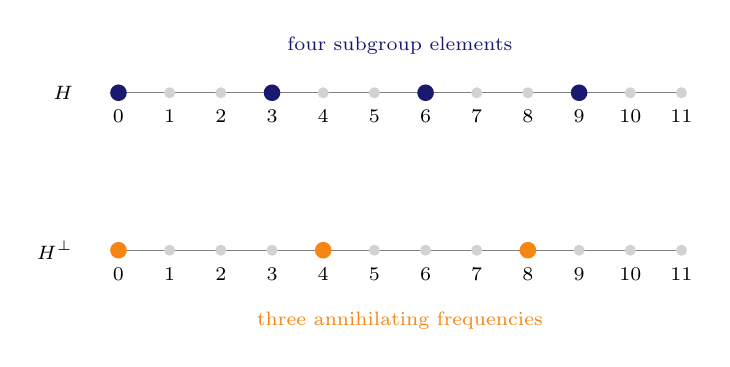
\begin{tikzpicture}[x=.65cm,y=1cm,every node/.style={font=\scriptsize}]
\node[anchor=east] at (-.7,1) {$H$};\node[anchor=east] at (-.7,-1) {$H^\perp$};
\draw[gray] (0,1)--(11,1);\draw[gray] (0,-1)--(11,-1);
\foreach \k in {0,...,11}{\fill[gray!35] (\k,1) circle (2pt);\fill[gray!35] (\k,-1) circle (2pt);\node[below] at (\k,.9) {$\k$};\node[below] at (\k,-1.1) {$\k$};}
\foreach \k in {0,3,6,9}{\fill[MidnightBlue] (\k,1) circle (3pt);}
\foreach \k in {0,4,8}{\fill[BurntOrange] (\k,-1) circle (3pt);}
\node[MidnightBlue] at (5.5,1.6) {four subgroup elements};
\node[BurntOrange] at (5.5,-1.9) {three annihilating frequencies};
\end{tikzpicture}
